\documentclass{beamer}
\usetheme{CambridgeUS}
\usecolortheme{dolphin}
\setbeamertemplate{page number in head/foot}{}
\usepackage[utf8]{inputenc}
\usepackage{dirtytalk,amssymb,tikz,mathtools,amsmath, empheq}
\usepackage{stackengine}
\usepackage{stmaryrd}
\usepackage{graphicx}
\usepackage[noend]{algpseudocode,algorithm}
\usepackage{resizegather}
\usetikzlibrary{automata, positioning}
\graphicspath{ {./images/} }
\tikzset{->, initial text=$$}
\DeclareMathAlphabet{\mathpzc}{OT1}{pzc}{m}{it}

\makeatletter
\algrenewcommand\ALG@beginalgorithmic{\footnotesize}
\makeatother

%Information to be included in the title page:
\title[CS 422 Programming Language Design]{K Semantics of Untyped Simple}

%\setbeameroption{hide notes} % Only slides
%\setbeameroption{show only notes} % Only notes
%\setbeameroption{show notes on second screen=right} % Both
%\setbeamertemplate{note page}{\pagecolor{yellow!5}\insertnote}\usepackage{palatino}
\setbeamerfont{caption}{size=\scriptsize}
\date{}

\begin{document}

\section{Review}

\begin{frame}{Simple Configuration}

\begin{figure}[h]
    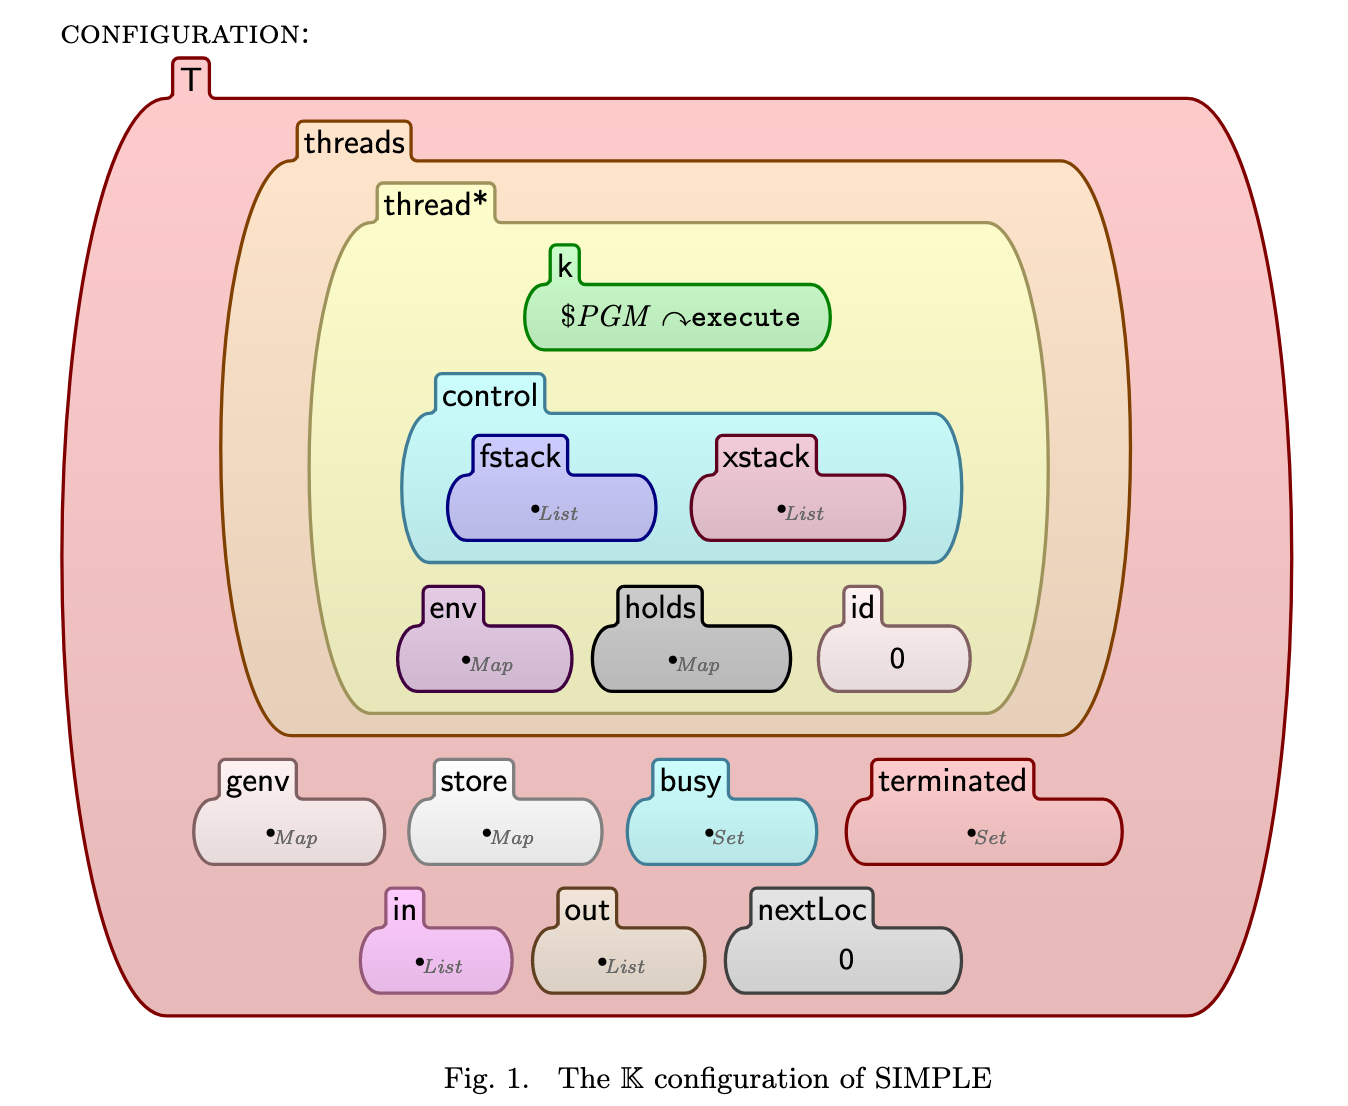
\includegraphics[width=0.6\textwidth]{configuration}
\end{figure}

\end{frame}

\begin{frame}{Starting execution}

\begin{figure}[h]
    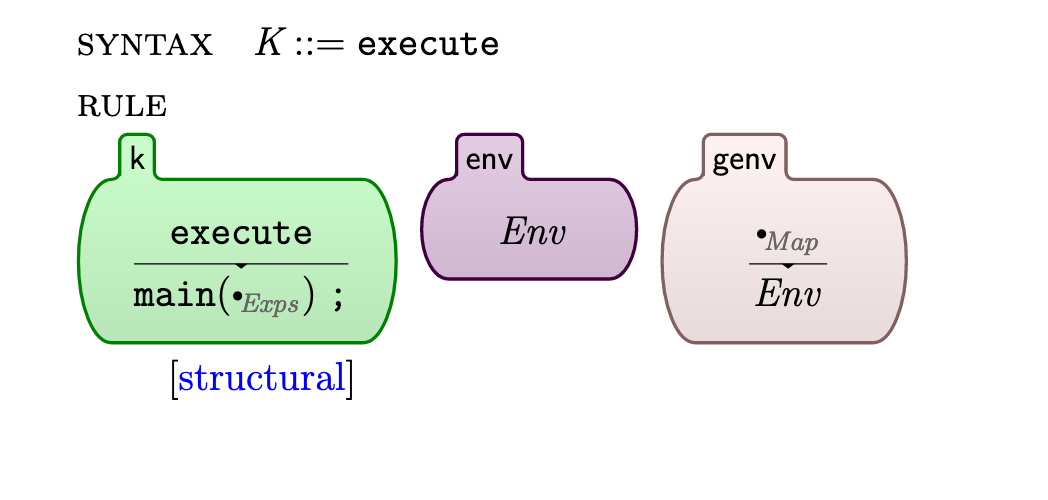
\includegraphics[width=0.6\textwidth]{execute}
\end{figure}
\end{frame}

\section{Simple Untyped Semantics}

\begin{frame}{Lookup}
\begin{figure}[h]
    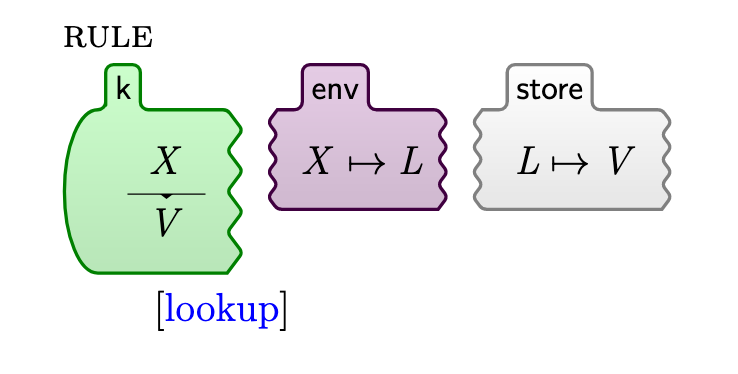
\includegraphics[width=0.6\textwidth]{lookup}
\end{figure}

\end{frame}

\begin{frame}{Increment}
\begin{figure}[h]
    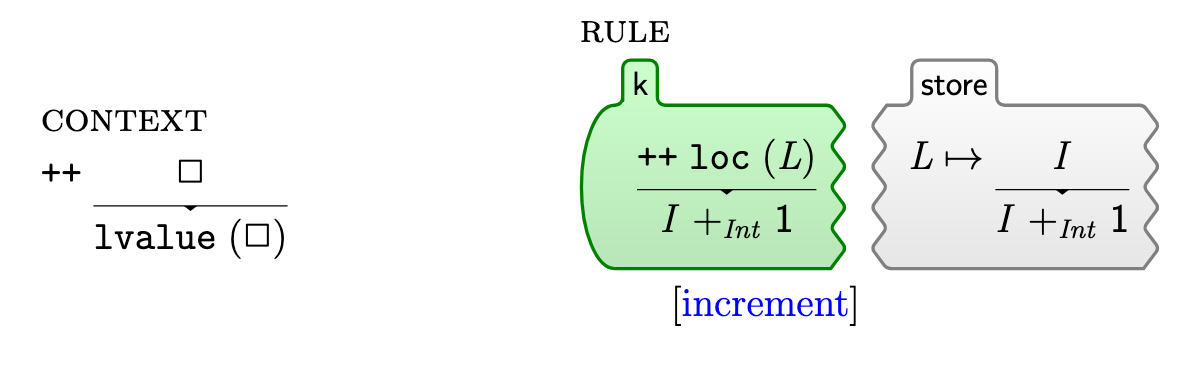
\includegraphics[width=0.6\textwidth]{increment}

    \begin{itemize}
        \item lvalue described in the next slide
        \pause
        \item Wrap \textit{increment Exp} into an auxilliary \text{lvalue} construct.
        \item Once \text{lvalue} evaluates to \textit location \text{loc(L)},
              perform increment.
    \end{itemize}
\end{figure}

\end{frame}

\begin{frame}{Increment (contd.)}
    \begin{figure}
        \centering
    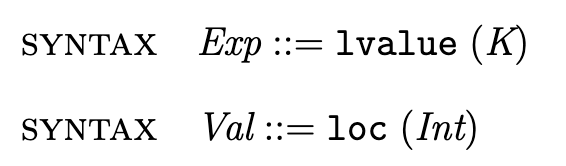
\includegraphics[width=0.4\textwidth]{lvalue-decl}
    \\
    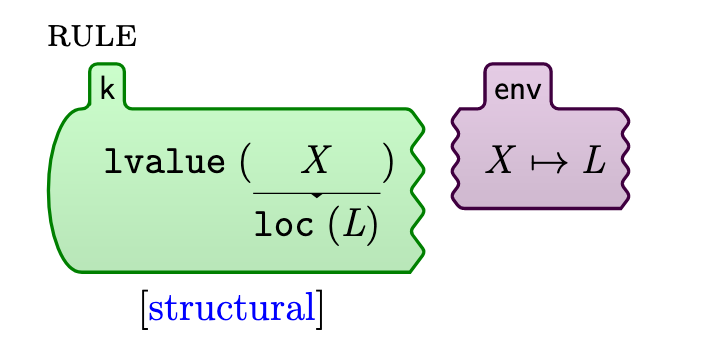
\includegraphics[width=0.4\textwidth]{lvalue-rules}
    \end{figure}
\end{frame}

\begin{frame}{Arithemic Operators}
    \begin{figure}
        \centering
    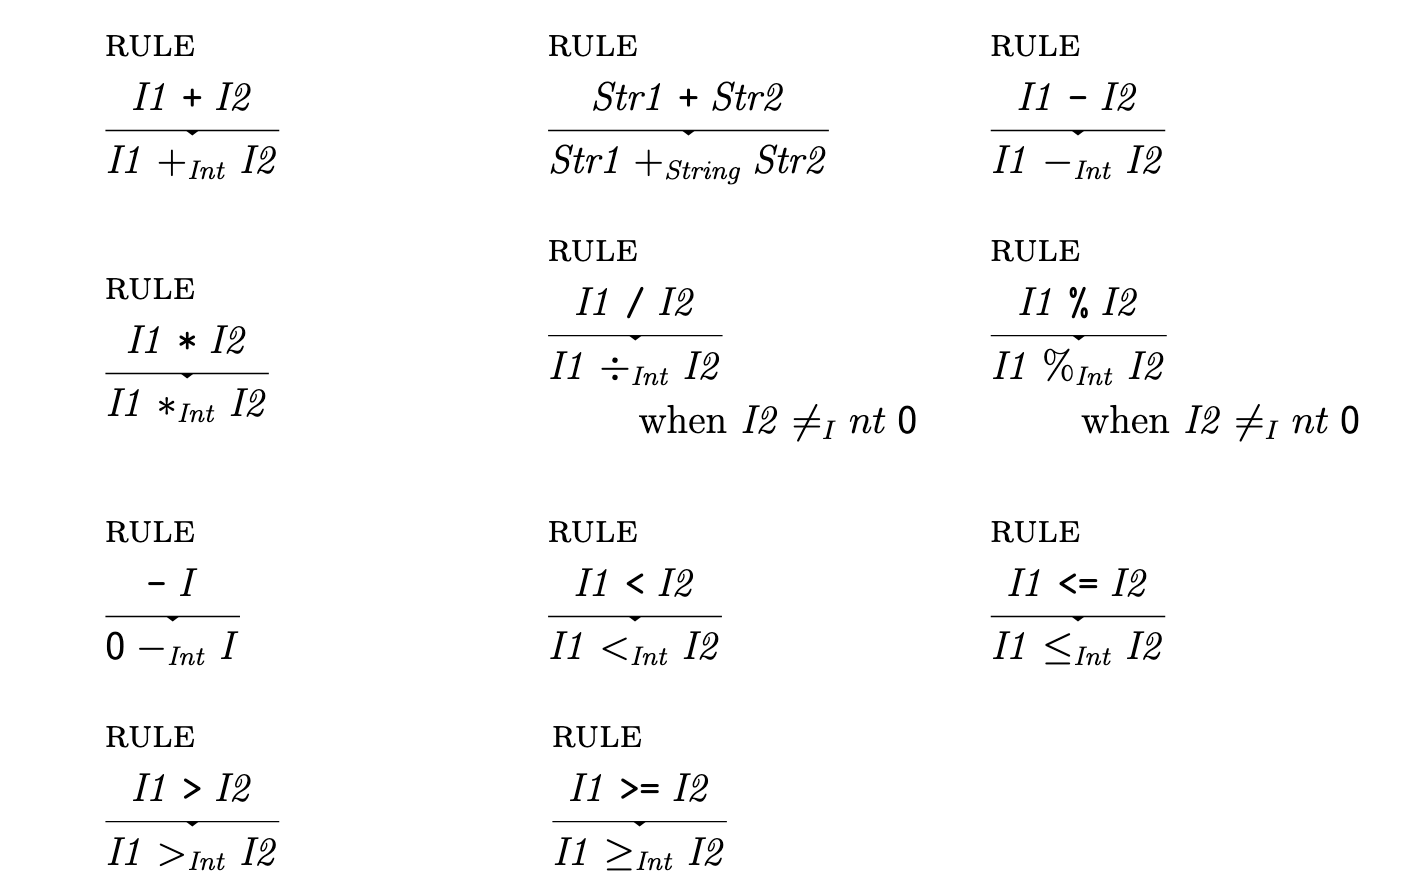
\includegraphics[width=0.5\textwidth]{arith-1}
    \\
    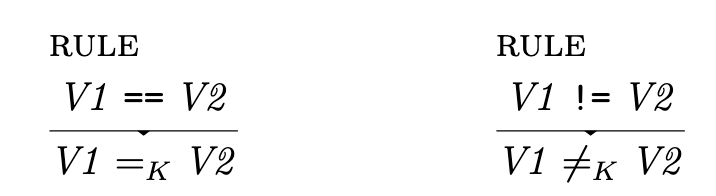
\includegraphics[width=0.3\textwidth]{arith-2}
    \end{figure}
\end{frame}

\begin{frame}{Boolean Operators}
    \begin{figure}
        \centering
    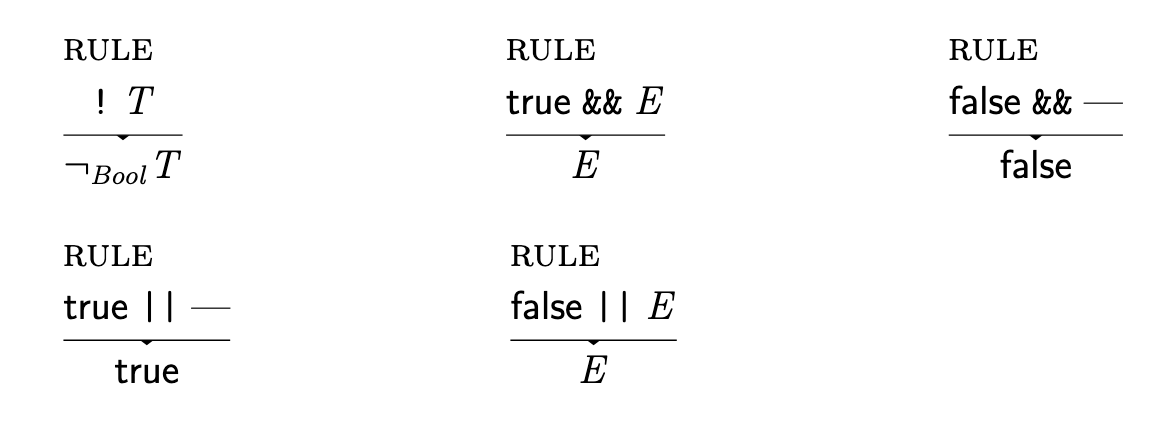
\includegraphics[width=0.5\textwidth]{bool-1}
    \end{figure}
\end{frame}
\begin{frame}{Array Lookup}
    \begin{figure}
        \centering
    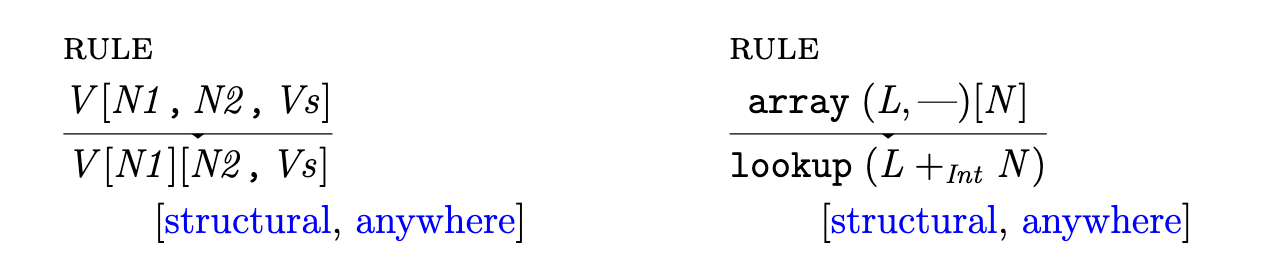
\includegraphics[width=0.6\textwidth]{array-lookup}
    \end{figure}

    \pause
    \begin{itemize}
        \item Lookup in an array - how are
            expressions handled in array offset?
        \pause
        \item what is \text{anywhere}?
        \pause
    \end{itemize}
\end{frame}


\begin{frame}{Array Lookup (contd.)}
    \begin{figure}
        \centering
    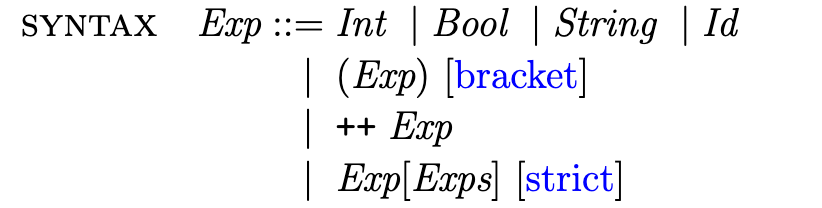
\includegraphics[width=0.4\textwidth]{array-syntax}
    \end{figure}

    \pause

    \begin{figure}
        \centering
    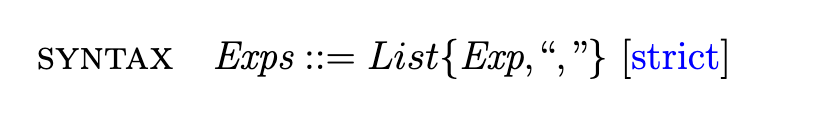
\includegraphics[width=0.6\textwidth]{exps-syntax}
    \end{figure}

    \pause
    \begin{figure}
        \centering
    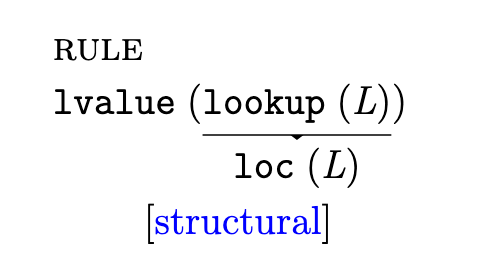
\includegraphics[width=0.4\textwidth]{lvalue-lookup}
    \end{figure}

\end{frame}
\begin{frame}{Array Size}
    \begin{figure}[H]
        \centering
    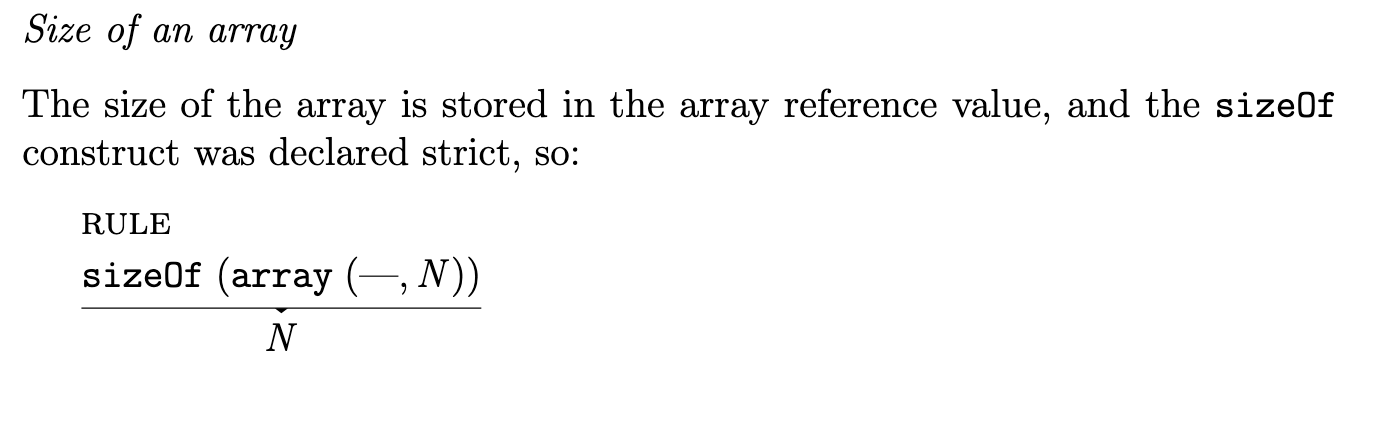
\includegraphics[width=0.8\textwidth]{array-sizeof}
    \end{figure}

\end{frame}

\begin{frame}{Function Calls}
    \begin{figure}[H]
        \centering
    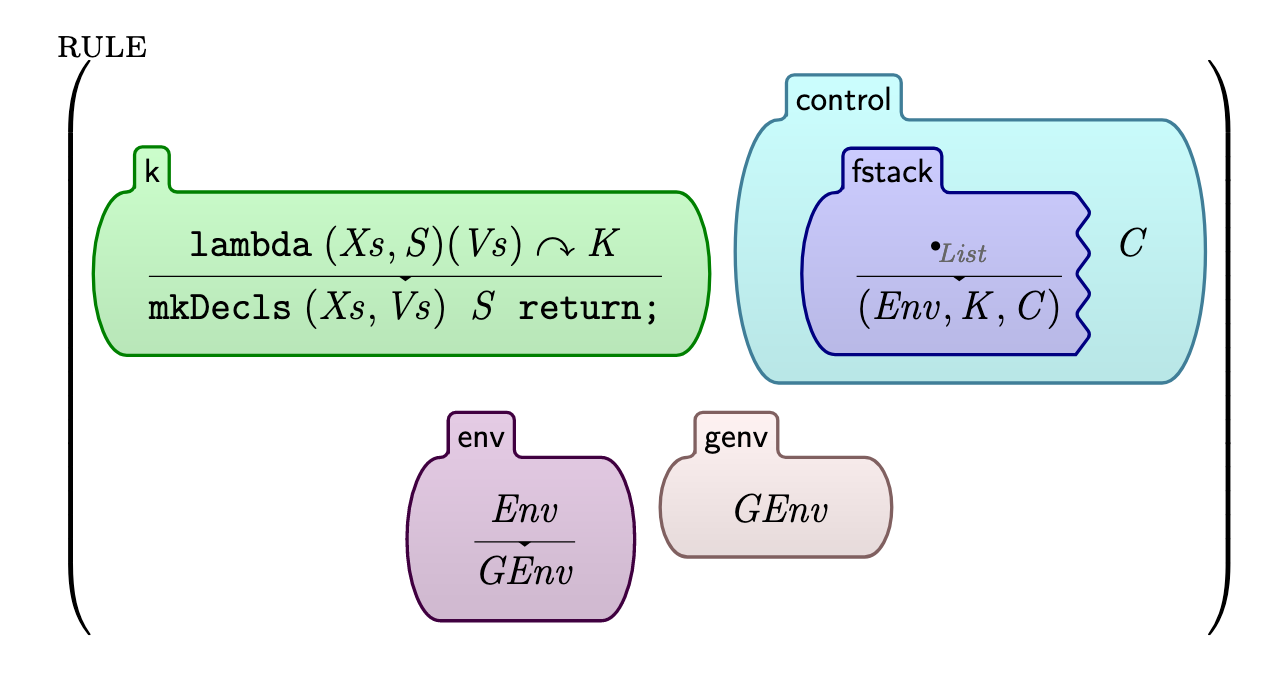
\includegraphics[width=0.6\textwidth]{fcall-1}
    \end{figure}
    \pause
    \begin{itemize}
        \item Switch to \textit{global environment}, where
            free variables in function are looked up.
    \end{itemize}

\end{frame}

\begin{frame}{Function Calls}
    \begin{figure}[H]
        \centering
    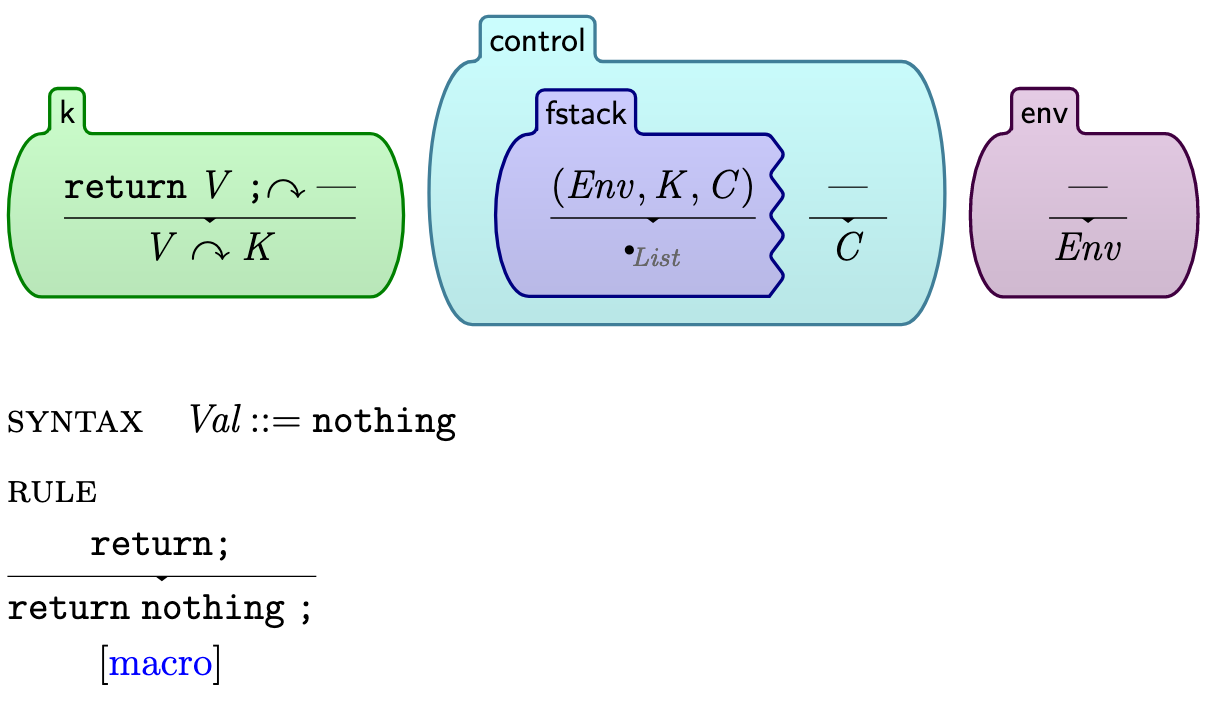
\includegraphics[width=0.6\textwidth]{fcall-2}
    \end{figure}
\end{frame}
\begin{frame}{Assignments \& Reads}
    \begin{figure}[H]
        \centering
    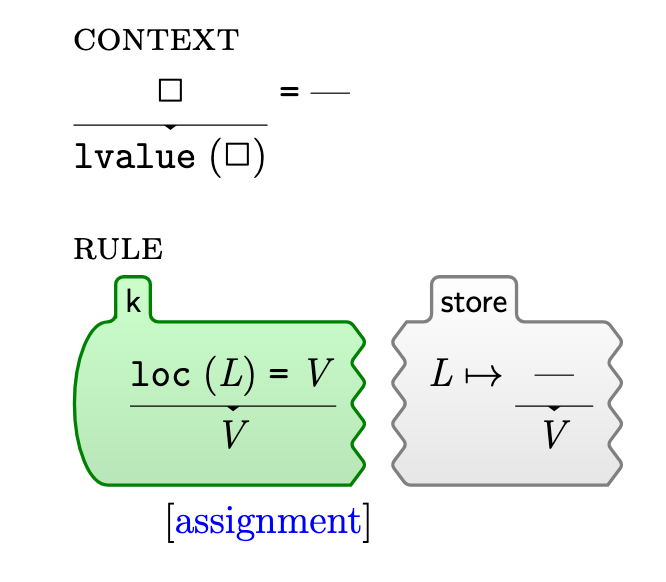
\includegraphics[width=0.4\textwidth]{assignment} \\
    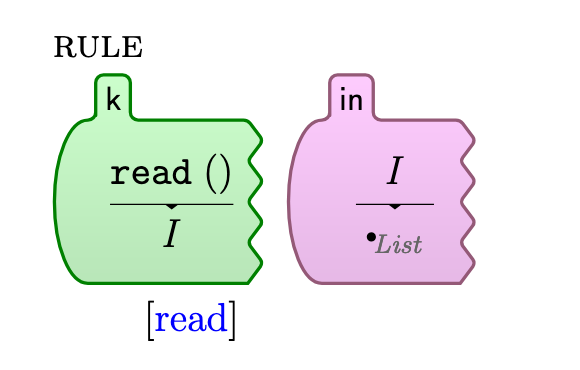
\includegraphics[width=0.4\textwidth]{read}
    \end{figure}
\end{frame}
\begin{frame}{Sequential Composition, Expressions \& Conditionals}
    \begin{figure}[H]
        \centering
    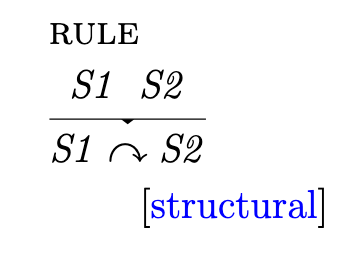
\includegraphics[width=0.3\textwidth]{seqcomp} \\
    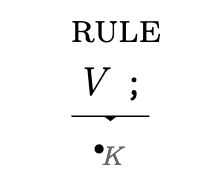
\includegraphics[width=0.2\textwidth]{expr} \\
    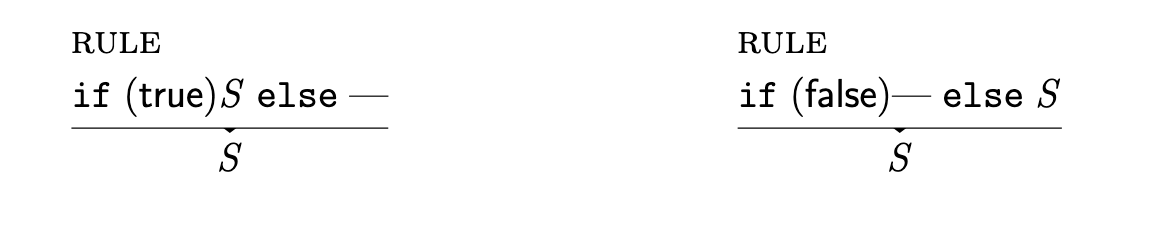
\includegraphics[width=0.7\textwidth]{cond}
    \end{figure}
\end{frame}
\begin{frame}{While \& Print}
    \begin{figure}[H]
        \centering
    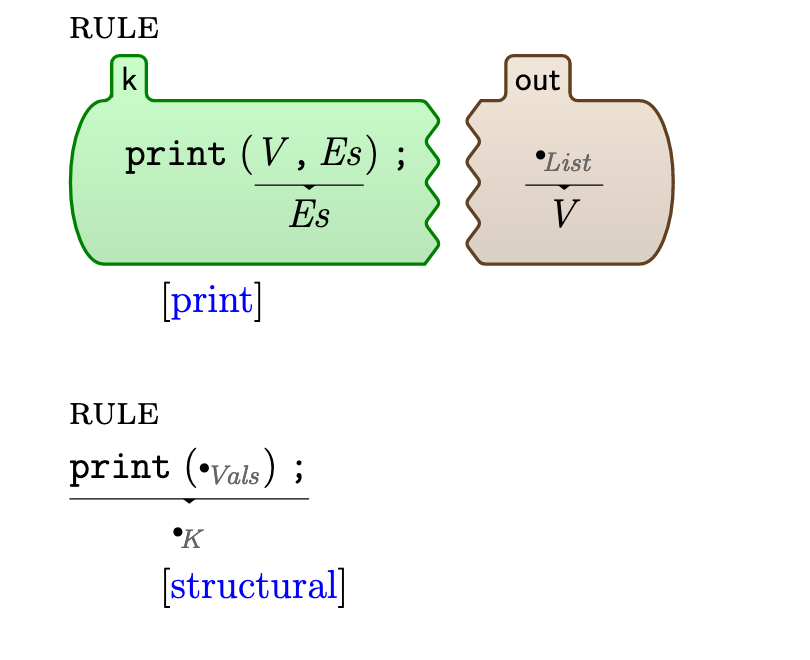
\includegraphics[width=0.3\textwidth]{while} \\
    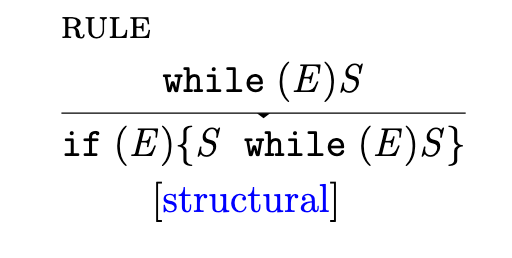
\includegraphics[width=0.2\textwidth]{print} \\
    \end{figure}
\end{frame}
\begin{frame}{Exception Handling}
    \begin{figure}[H]
        \centering
    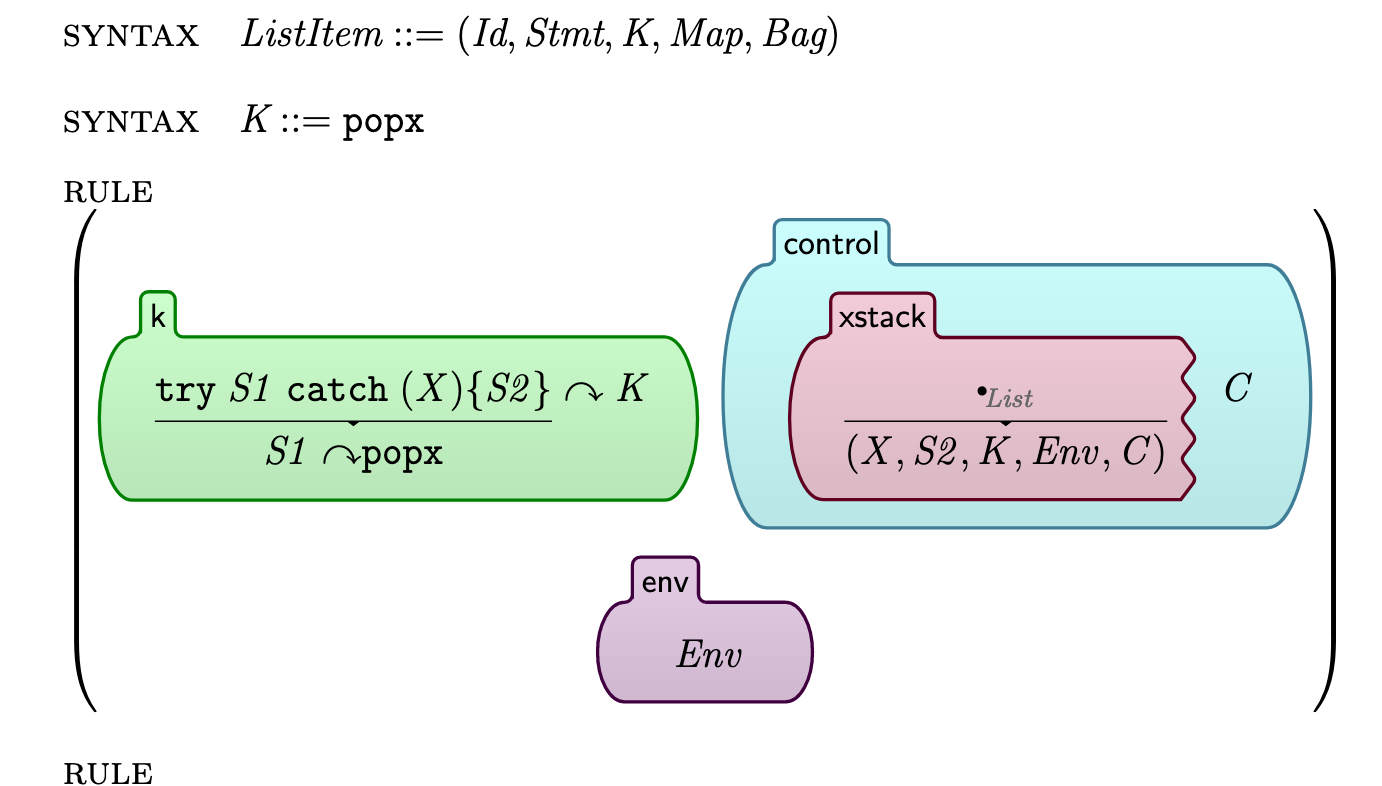
\includegraphics[width=0.6\textwidth]{trycatch} \\
    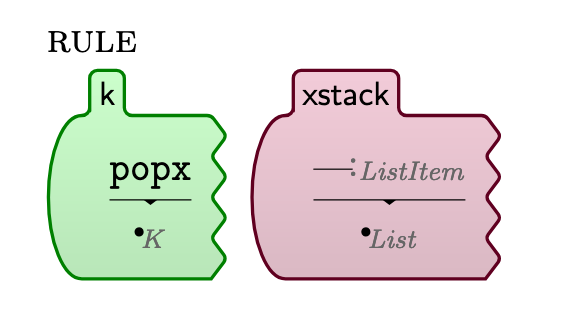
\includegraphics[width=0.3\textwidth]{pop} \\
    \end{figure}
\end{frame}
\begin{frame}{Exception Handling (contd.)}
    \begin{figure}[H]
        \centering
    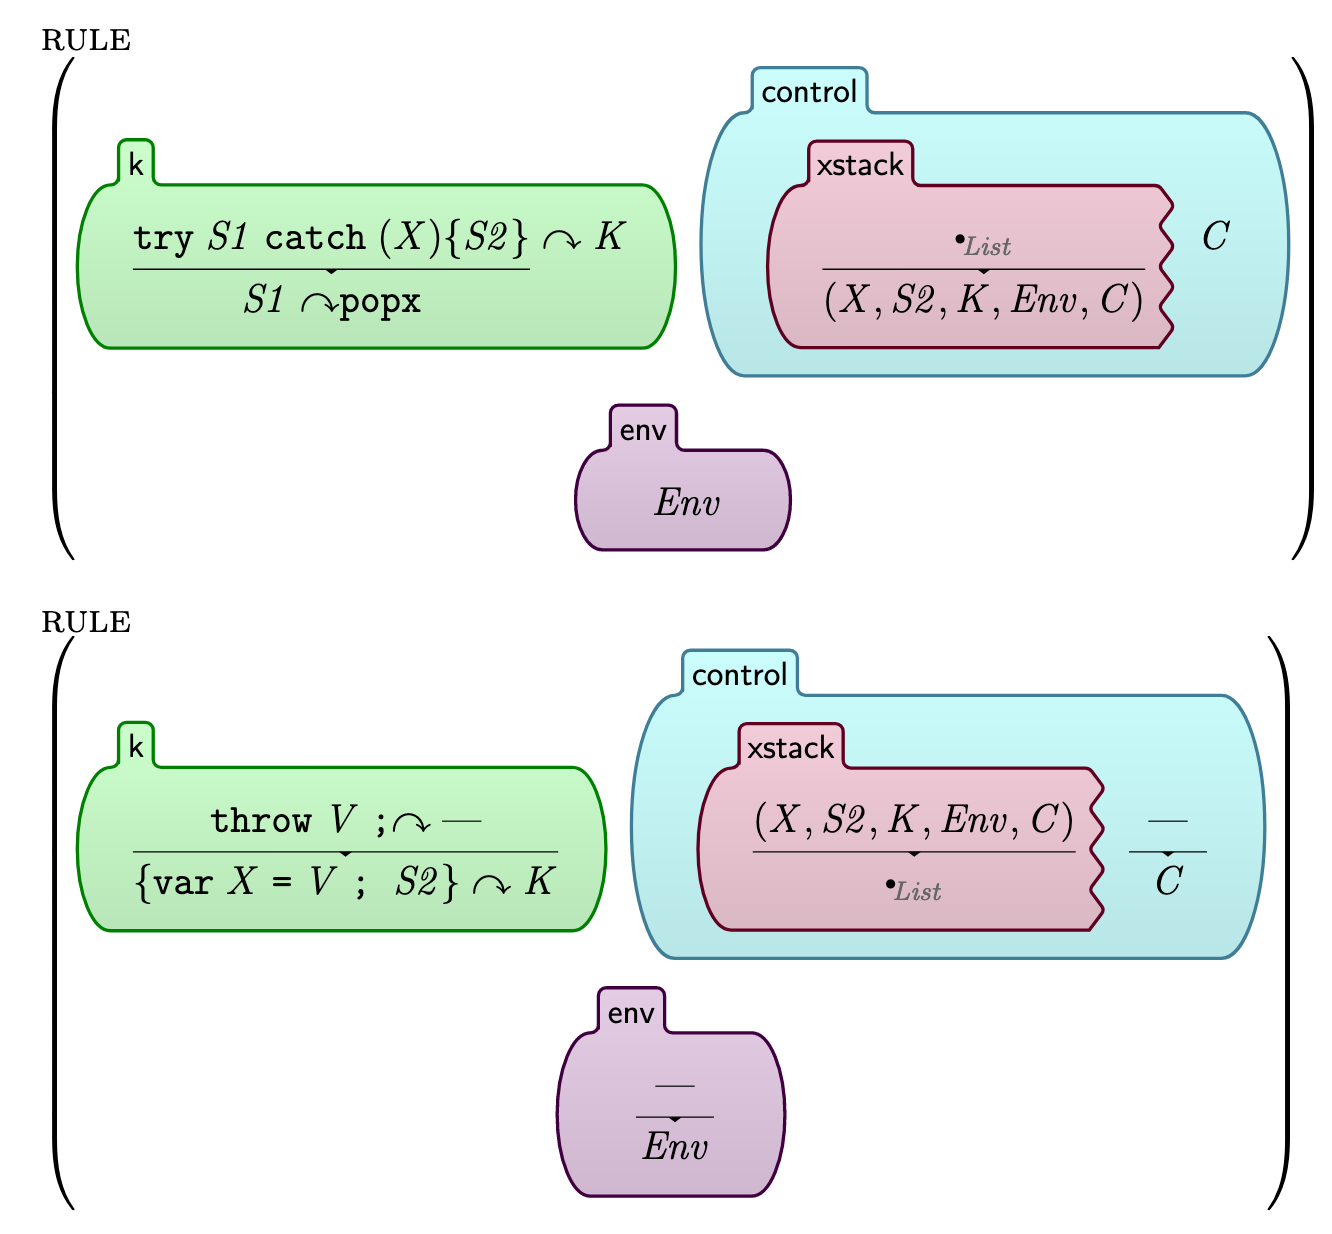
\includegraphics[width=0.6\textwidth]{throw} \\
    \end{figure}
\end{frame}

\begin{frame}{Concurrency}{Spawn}
    \begin{figure}[H]
        \centering
    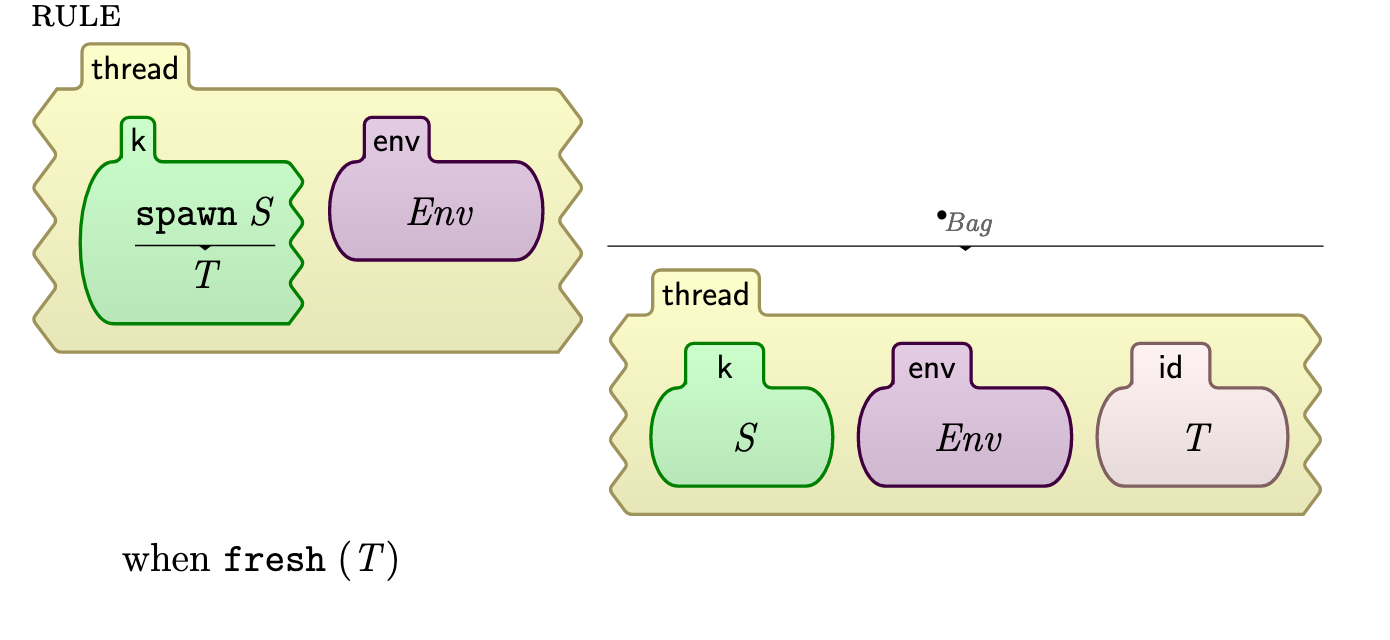
\includegraphics[width=0.6\textwidth]{thread-creation} \\
    \end{figure}
\end{frame}
\begin{frame}{Concurrency}{Termination \& Joining}
    \begin{figure}[H]
        \centering
    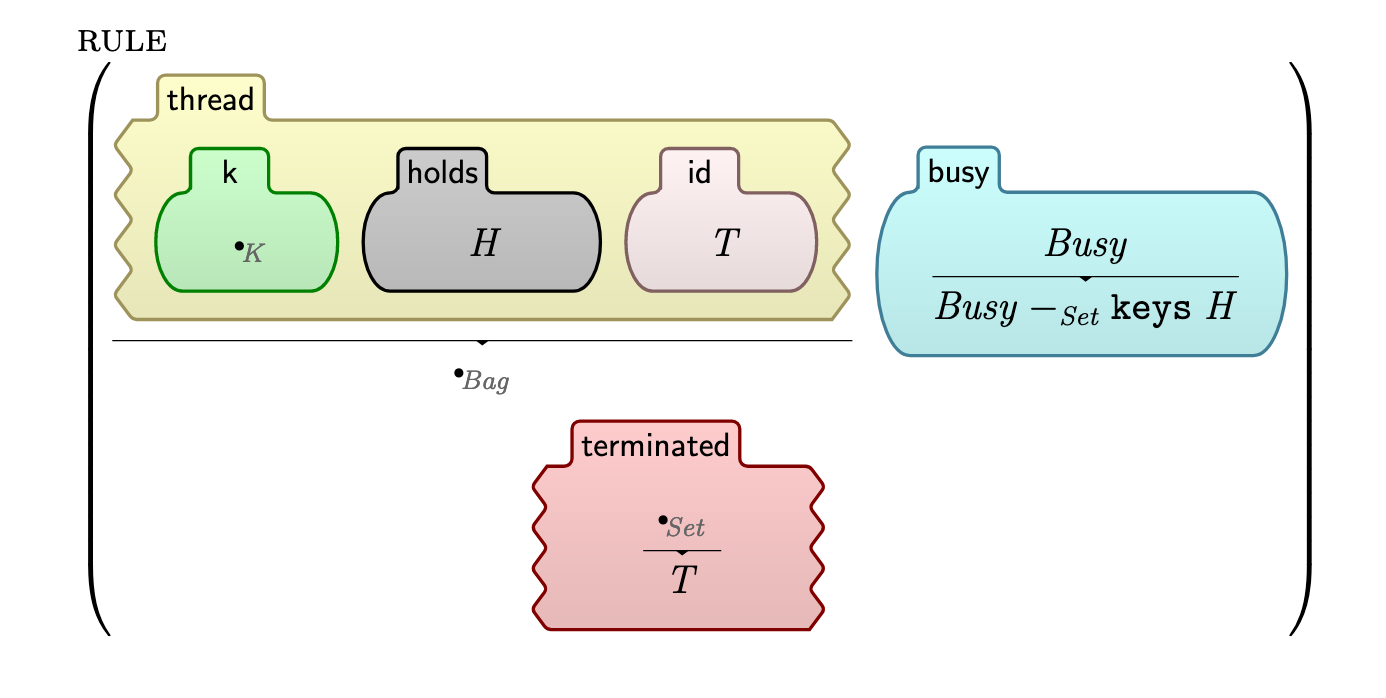
\includegraphics[width=0.6\textwidth]{thread-termination} \\
    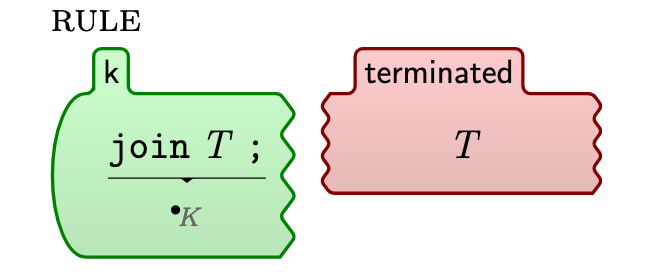
\includegraphics[width=0.3\textwidth]{thread-join} \\
    \end{figure}
\end{frame}
\begin{frame}{Concurrency}{Acquire Locks}
    \begin{figure}[H]
        \centering
    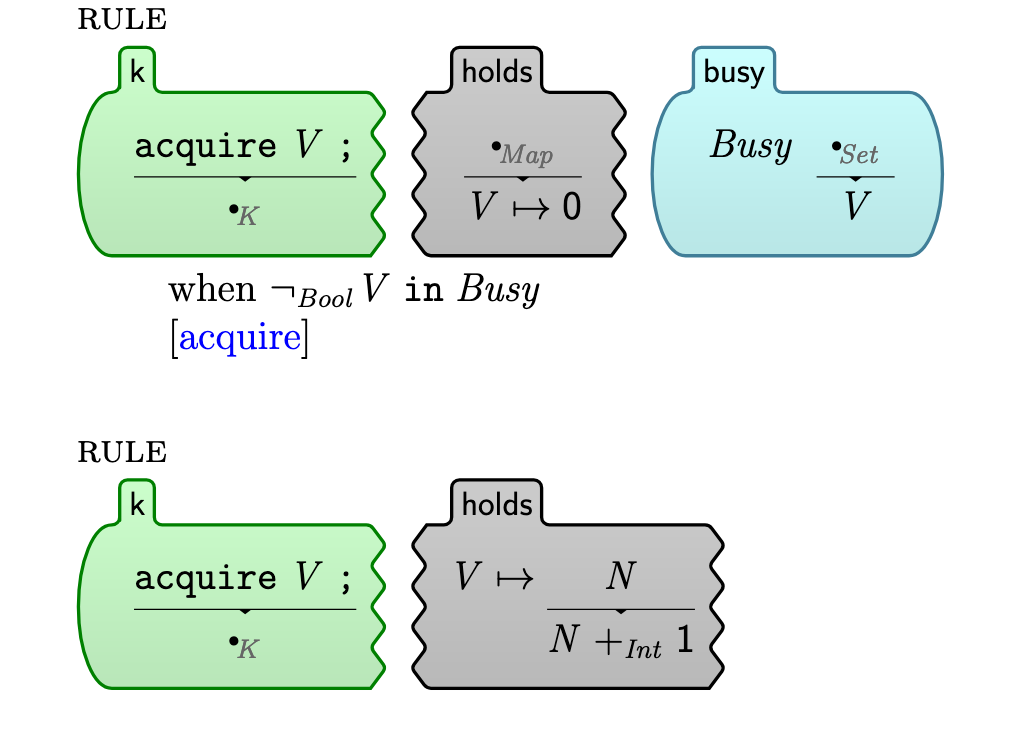
\includegraphics[width=0.6\textwidth]{acquire-lock.png} \\
    \end{figure}
    \pause
    \begin{itemize}
        \item Assume re-entrace. Same thread can acquire a lock
            again.
    \end{itemize}
\end{frame}
\begin{frame}{Concurrency}{Release Locks}
    \begin{figure}[H]
        \centering
    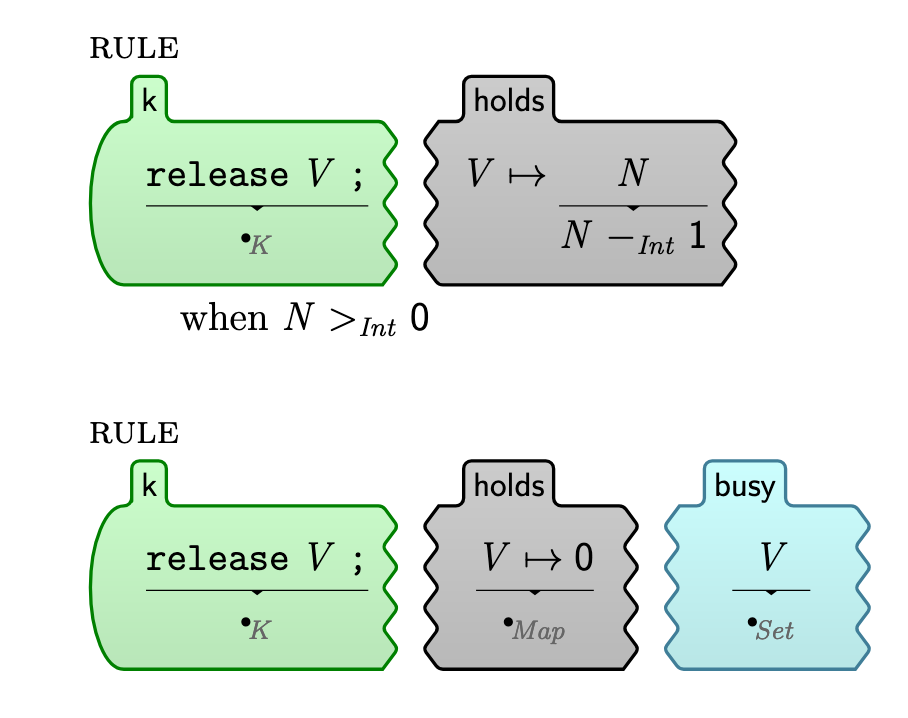
\includegraphics[width=0.6\textwidth]{release-lock.png} \\
    \end{figure}
    \pause
    \begin{itemize}
        \item A lock is considered release only when $n$ release
            calls match with $n$-acquires calls.
    \end{itemize}
\end{frame}
\begin{frame}{Concurrency}{Rendezvous}
    \begin{figure}[H]
        \centering
    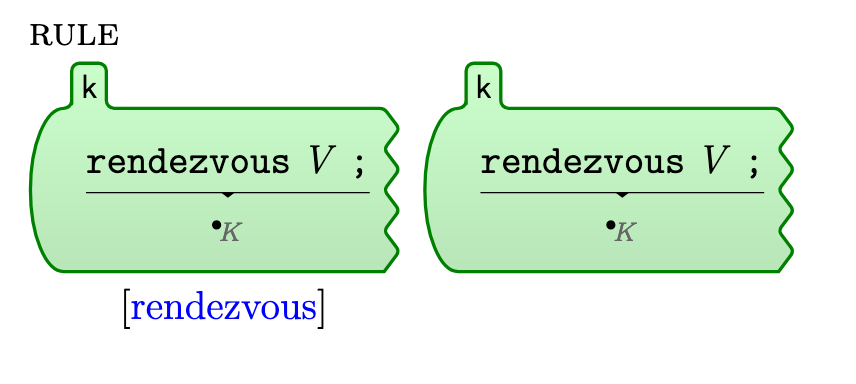
\includegraphics[width=0.6\textwidth]{rendezvous.png}
    \end{figure}
\end{frame}

\begin{frame}{Auxilliary Constructs}{Declarations, Lookups \& Restoring Environments}
    \begin{figure}[H]
        \centering
    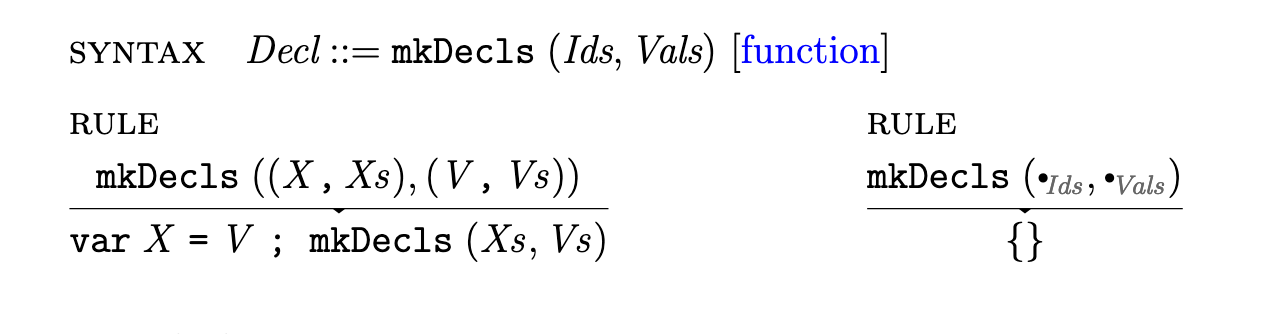
\includegraphics[width=0.4\textwidth]{declarations} \\
    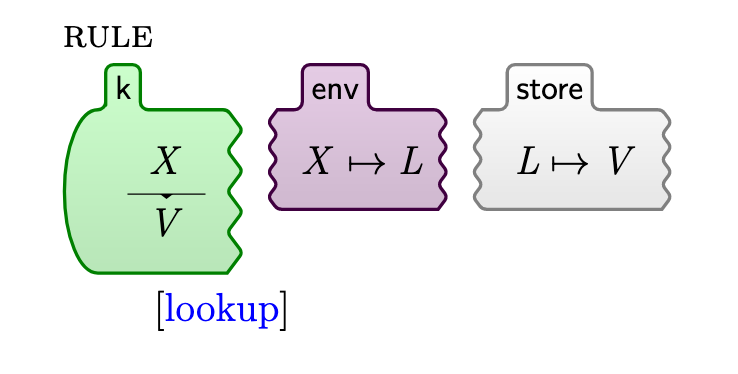
\includegraphics[width=0.4\textwidth]{lookup}
    \end{figure}
\end{frame}

\begin{frame}{Auxilliary Constructs}{Restoring Environments}
    \begin{figure}[H]
        \centering
    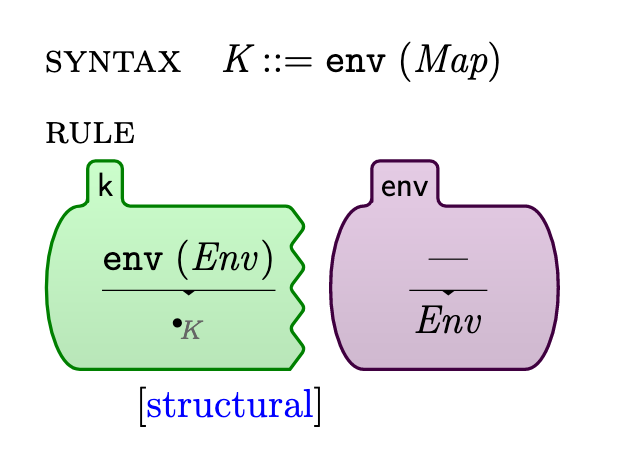
\includegraphics[width=0.4\textwidth]{restore-env}
    \end{figure}
\end{frame}
% \begin{frame{Simple Configuration}}
%     \begin{itemize}
%         \item A textit{Global Environment} and
%     \end{itemize}
% \end{frame}

\end{document}

